\begin{algorithm}[t]
	\caption{\astarix including heuristic function.}\label{TRIEalg:astarix}
	\begin{algorithmic}[1]
		\State $\RG$: Reference graph \label{TRIElin:reference}
		\Comment Global variables
		\State $d$: Upcoming sequence length \label{TRIElin:d}
		\Statex
		\Function{AStarix}{$q\colon \text{Query}$} \label{TRIElin:astarix}
			\State $\AG \gets \Call{DefineAlignmentGraph}{\RG, q}$
			\Comment Following \cref{TRIEsec:task}
			\State $S \gets \{\langle v,i \rangle \in \AGV \mid i=0 \}$ \label{TRIElin:starts}
			\Comment Sources: no letter matched
			\State $T \gets \{\langle v,i \rangle \in \AGV \mid i=|q| \}$
			\Comment Targets: all letters matched
			\State \Return $\Call{\A}{\AG, S, T, \textsc{Heuristic}}$
			\Comment \A provided in \cref{TRIEapp:astar} \label{TRIElin:ret}
		\EndFunction
		\Statex
		\Function{Heuristic}{$\langle u, i \rangle\colon \text{State}$} \label{TRIElin:heuristic-start}
		\Comment Heuristic: Cost of upcoming sequence
			\State $d' \gets \min(d, |q|-i)$
			\Comment Actual length of upcoming sequence
			\State $s \gets q[i:i+d']$ \label{TRIElin:s}
			\Comment Upcoming sequence (next $d$ letters after current)
			\State \Return $\Call{$h$}{u, s}$
			\label{TRIElin:align-upcoming}
			\Comment Cost of aligning $s$ to $\RG$ starting from $u$
		\EndFunction \label{TRIElin:heuristic-end}
		\Statex
		\Function{$h$}{$u, s$}
		\Comment Cost of aligning $s$ starting from $u$
			\State \Return $\Call{RecursiveAlign}{u, s, 0.0, \infty}$
			\Comment Simple branch-and-bound \label{TRIElin:recursive-align}
		\EndFunction
	\end{algorithmic}
\end{algorithm}
\subsection{Background: General \A algorithm} \label{subsec:general-astar}
Given a weighted graph $G=(V,E)$ with $E \subseteq V \times V \times
\mathbb{R}_{\geq 0}$, the \A algorithm (abbreviated as \A) searches for the
shortest path from sources $S \subseteq V$ to targets $T \subseteq V$. It is an
extension of Dijkstra's algorithm that additionally leverages a \emph{heuristic
function} $h \colon V \to \mathbb{R}_{\geq 0}$ to decide which paths to explore
first.
%
If $h(u) \equiv 0$, \A is equivalent to Dijkstra's algorithm.
%
We provide an implementation of \A and Dijkstra in \cref{app:astar}, but do not
assume knowledge of either algorithm in the following.
%
At a high level, \A maintains the set of all \emph{explored} states, initialized
with the set of sources $S$. Then, \A iteratively \emph{expands} the explored
state with lowest estimated cost by exploring all its neighbors, until it finds
a target. Here, the cost for node $u$ is estimated by the distance from source, called $g(u)$, plus the estimate from the heuristic $h(u)$.


\para{Heuristic Function}
The heuristic function $h(u)$ estimates the
cost $h^*(u)$ of a shortest path in $G$ from $u$ to a target $t \in T$. Intuitively, a
good heuristic correlates well with the distance from $u$ to $t$.

To ensure that \A indeed finds the shortest path, $h$ should be
\emph{optimistic}:

\begin{definition}[Optimistic heuristic] A heuristic $h$ is \textit{optimistic}
    if it provides a lower bound on the distance to the closest target: $\forall u. h(u) \leq h^*(u)$.
\end{definition}

While any optimistic $h$ ensures that \A finds optimal
alignments~\cite[Res.~3]{dechter_generalized_1985}, the specific choice of $h$
is critical for performance. In particular, decreasing the error $\delta(u) =
h^*(u)-h(u)$ can only improve the performance of
\A~\cite[Res.~6]{dechter_generalized_1985}. Thus, a key contribution of ours is a domain-specific heuristic $h$.


\subsection{\astarix: Instantiating \A} \label{TRIEsubsec:astarix-heuristic}
\cref{TRIEalg:astarix} shows an unoptimized version of \astarix and its heuristic
function.
%
\astarix expects a reference graph (\cref{TRIElin:reference}) and a query
(\cref{TRIElin:astarix}) as input, and returns an optimal alignment (\cref{TRIElin:ret})
by searching for a shortest path from $S$ to $T$ in the alignment graph $\AG$.
It is parameterized by hyper-parameters ($d$ in \cref{TRIElin:d}, more in
\cref{TRIEsec:optimizations}) and edit costs (implicitly provided).

The function \textsc{Heuristic}
(\crefrange{TRIElin:heuristic-start}{TRIElin:heuristic-end}) computes a lower bound on
the remaining cost of a best alignment: the minimum cost $h(u,s)$ of aligning
the \emph{upcoming sequence} $s$ (where $\lvert s \rvert \leq d$) starting from
node $u$. Importantly, $s$ is limited to the next $d' \leq d$ letters of $q$,
starting from query position $i$. Thus, computing $h(u,s)$ is substantially
cheaper than aligning all remaining letters of $q$.

To compute $h(u,s)$ we leverage a simple branch-and-bound algorithm, provided in
\cref{TRIEapp:recursive-align}. In the following, for convenience, we refer to the
heuristic as $h$ (which is parameterized by $(u,s)$) instead of
\textsc{Heuristic} (which is parameterized by $\langle u, i \rangle$). Further,
we say that $h$ is optimistic if $h(u,s)$ is a lower bound on the cost for
aligning all remaining letters (\ie, $q[i:|q|]$) starting from node $u$ (note
that $s$ is a prefix of $q[i:|q|]$).

\begin{samepage}
\begin{thm} \label{TRIEthm:optimistic}
	$h$ is optimistic.
\end{thm}
\begin{proof}
$h$ only considers the next $d'$ letters of $q$ instead of all
remaining letters. Since all costs are non-negative, the theorem follows.
\end{proof}
\end{samepage}

\begin{figure}[t]
	\centering
	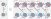
\includegraphics[width=0.9\columnwidth]{\dir/figs/heuristic}
	\caption{The benefit of using our heuristic over \dijkstra. Alignment graph
	$\AG[``\texttt{ATAA}"]$ (right) is based on reference graph $\RG$ (left),
	but omits insertion and deletion edges for simplicity. The pink boxes $g+h$
	indicate the distance from the sources $S=\{\langle u,0 \rangle, \langle v,0
	\rangle \}$ (in $g$) and the cost of aligning the next $d=2$ letters (in
	$h$). \dijkstra (resp. \A) expands states circled in
	\textcolor{my-full-blue}{blue} (resp.
	\textcolor{my-full-red}{dashed red}).}
	\label{TRIEfig:heuristic-benefit}
\end{figure}

\para{Benefit of \A Heuristic over \dijkstra} \label{TRIEpara:heuristic-benefits}
\cref{TRIEfig:heuristic-benefit} shows the benefit of using our heuristic function
compared to \dijkstra. Here, \dijkstra expands states based on their distance
$g$ from the origin nodes $\st{u}{0}$ and $\st{v}{0}$. Hence, depending on
tie-breaking, \dijkstra may expand all states with $h \leq 1$, as shown in
\cref{TRIEfig:heuristic-benefit}. By contrast, \A chooses the next state to expand
by the sum of the distance from the origin $g$ and the heuristic $h$, expanding
only states with $g+h \leq 1$.

\para{Memoization} \label{TRIEpara:memoization}
Recall that the return value of $h$ in \cref{TRIElin:heuristic-start} only depends
on $u$ and the upcoming sequence $s$ (which in turn depends on $i$ and $d$).
Thus, $h(u,s)$ can be reused for different positions across different queries in
$\Oh(1)$ time, if it was computed for a previous query.